\begin{table}
    \centering
        \renewcommand\arraystretch{1.}
        % \vskip -0.1cm
        \caption{\textbf{Quantitative Main Results.} Please refer to \S\ref{sec:datasets_metrics} and Appx.\ref{app:datasets_metrics} for detailed task formulations and metric computations.}
        \vskip -0.1cm
        \scalebox{.57}{
        \begin{tabular}{l|cc|cc|cc|ccc}
            \toprule
            \multirow{2}{*}{\textbf{Method}} & \multicolumn{4}{c|}{\textbf{Point-wise}} &
            \multicolumn{2}{c|}{\textbf{Pair-wise}} & \multicolumn{3}{c}{\textbf{Group-wise}} \\
            \cmidrule{2-5} \cmidrule{6-7} \cmidrule{8-10}
            & Acc$_2$ & F1$_2$ & Acc$_3$ & F1$_3$ & Acc$_{\rm easy}$ & Acc$_{\rm hard}$ & Best & Lis & Acc \\
            \midrule
            CoT & 40.55 & 35.98 & 34.56 & 27.86 & 46.51 & 40.50 & 36.63 & 57.59 & 6.98  \\
            RAG & 42.40 & 38.29 & 35.48 & 28.45 & 44.19 & 39.00 & 34.30 & 57.88 & 7.56 \\
            GraphEval & 54.83 & 45.71 & 53.46 & 33.03 & 43.60& 44.50 & 20.93 & 57.70 & 2.33 \\
            ResearchAgent & 59.48 & 56.44 & 54.84 & 39.81 & 52.32 & 43.00 & 40.12 & 66.52 & 8.14 \\
            InternAgent & 60.37 & 60.12 & 56.68 & 43.05 & 62.65 & 59.50 & 41.28 & 68.46 & 10.47 \\
            ScholarEval  & 65.44 & 65.02 & 61.75 & 58.38 & 74.42 & 60.00 & 49.42 & 70.13 & 14.53 \\
            \midrule
            \textbf{\ours} & \textbf{75.58} & \textbf{75.74} & \textbf{73.73} & \textbf{74.56} & \textbf{80.81} & \textbf{63.00} & \textbf{65.12} & \textbf{76.03} & \textbf{22.09} \\
            \bottomrule
        \end{tabular}
        }
        \vskip -0.25in
        \label{tab:main_number}
    % \end{minipage}
\end{table}

\begin{table*}
    \centering
    \renewcommand\arraystretch{.9}
    \vskip -0.1cm
    \caption{\textbf{Qualitative Main Results} by using o4-mini as the judge. \textit{Rationality} measures the logical soundness; \textit{Supportiveness} indicates whether the analysis is adequately backed by evidence; \textit{Depth} assesses the thoroughness of the review; \textit{Constructiveness} reflects the usefulness and feasibility of the suggestions; \textit{Overall Quality} provides a holistic judgment of the entire content.}
    \vskip -0.2cm
    \scalebox{.85}{
    \begin{tabular}{l|cc|cc|cc|cc|cc}
        \toprule
        \multirow{1}{*}{\textbf{Baselines}} & \multicolumn{2}{c|}{\textbf{Rationality}} &
        \multicolumn{2}{c|}{\textbf{Supportiveness}} & \multicolumn{2}{c|}{\textbf{Depth}} & \multicolumn{2}{c|}{\textbf{Constructiveness}} & \multicolumn{2}{c}{\textbf{Overall Quality}} \\
        \cmidrule{2-3} \cmidrule{4-5} \cmidrule{6-7} \cmidrule{8-9} \cmidrule{10-11} 
        \textbf{{\ours} vs.} & \textbf{Win(\%)} & \textbf{Lose(\%)} & \textbf{Win(\%)} & \textbf{Lose(\%)} & \textbf{Win(\%)} & \textbf{Lose(\%)} & \textbf{Win(\%)} & \textbf{Lose(\%)} & \textbf{Win(\%)} & \textbf{Lose(\%)} \\
        \midrule
        CoT & \textbf{88.48} & 9.22 & \textbf{92.17} & 2.76 & \textbf{93.09} & 6.91 & \textbf{89.77} & 9.77 & \textbf{90.70} & 7.83 \\
        RAG & \textbf{87.10} & 11.98 & \textbf{87.56} & 11.52 & \textbf{92.63} & 6.45 & \textbf{87.10} & 9.68 & \textbf{90.32} & 8.37 \\
        ResearchAgent & \textbf{86.18} & 12.44 & \textbf{86.18} & 7.37 & \textbf{90.32} & 8.29 & \textbf{88.94} & 9.68 & \textbf{89.86} & 8.29 \\
        InternAgent & \textbf{83.41} & 15.67 & \textbf{87.10} & 9.22 & \textbf{91.24} & 7.37 & \textbf{82.03} & 16.59 & \textbf{85.71} & 12.90 \\
        ScholarEval & \textbf{67.28} & 28.11 & \textbf{61.75} & 32.72 & \textbf{70.51} & 28.11 & \textbf{84.79} & 14.29 & \textbf{71.89} & 25.81\\
        \bottomrule
    \end{tabular}
    }
    \vskip -0.1in
    \label{tab:main_llm}
\end{table*}

% \vskip -0.2cm
\section{Experimental Settings}
\subsection{Datasets and Metrics.}
\label{sec:datasets_metrics}
\textbf{Point-wise Dataset.}
To curate high-quality ideas for evaluation, we extract ideas from authoritative peer-reviewed papers to construct our test dataset.
Specifically, we crawl NeurIPS25 and ICLR25 papers from OpenReview and partition them into four strata according to their final decisions (Reject, Poster, Spotlight, Oral), from which we perform stratified sampling.
We specially include every submission track within each stratum to ensure diversity.
We apply our extraction agent $\boldsymbol{\mathcal{M}}_e$ to harvest ideas from each paper, followed by manual correction and verification, finally yielding 217 point-wise samples, which we mark as $\boldsymbol{\mathcal{D}}_\textrm{point}$.
We design two classification tasks of different difficulty:
\textit{i) Binary classification}, predicting whether an idea can be accepted (Reject vs. others);
\textit{ii) Ternary classification}, where we group Spotlight and Oral into a single class called Highlight.
We use Accuracy and macro F1 as the evaluation metrics.

\textbf{Pair-wise and Group-wise Datasets.}
To construct idea groups with similar topics, we use each idea in $\boldsymbol{\mathcal{D}}_\textrm{point}$ as a query to retrieve similar papers from the crawled paper pool.
We select the paper with the highest similarity for each stratum to form a group, so that the ideas in each group can be automatically ranked according to their labels.
We finally obtain 172 group-wise instances as $\boldsymbol{\mathcal{D}}_\textrm{group}$.
We define two group-wise tasks:
\textit{i) Best selection} to identify the best idea within each group, and  
\textit{ii) Ranking} to produce the exact full ranking list.  
We evaluate best selection by Accuracy and ranking task via Longest Increasing Subsequence Match and Accuracy.
Pair-wise idea comparison is also highly practical in everyday research workflows.
So we sample idea pairs from $\boldsymbol{\mathcal{D}}_\textrm{group}$ and split them into two difficulty levels:
\textit{i) Easy}, where the two ideas exhibit a clear label gap (e.g., Reject vs. Highlight);  
\textit{ii) Hard}, where the labels are adjacent (e.g., Poster vs. Highlight, Reject vs. Poster).
After filtering, we construct a dataset $\boldsymbol{\mathcal{D}}_{\textrm{pair}}$ comprising 372 samples, including 172 easy pairs and 200 hard pairs.
We directly use Accuracy to evaluate pair-wise tasks.
Further details about dataset construction and metrics are provided in Appx.\ref{app:datasets_metrics}.

\begin{figure*}
    \begin{subfigure}[b]{0.2\textwidth}
        \centering
        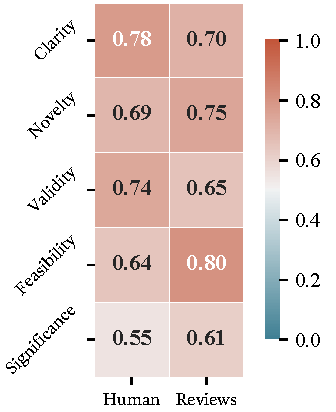
\includegraphics[width=.85\textwidth]{figure/human_reviews_heatmap.pdf}
        % \caption{\textbf{Human Evaluation.}}
        \label{fig:human}
    \end{subfigure}
    \begin{subfigure}[b]{0.8\textwidth}
        \centering
        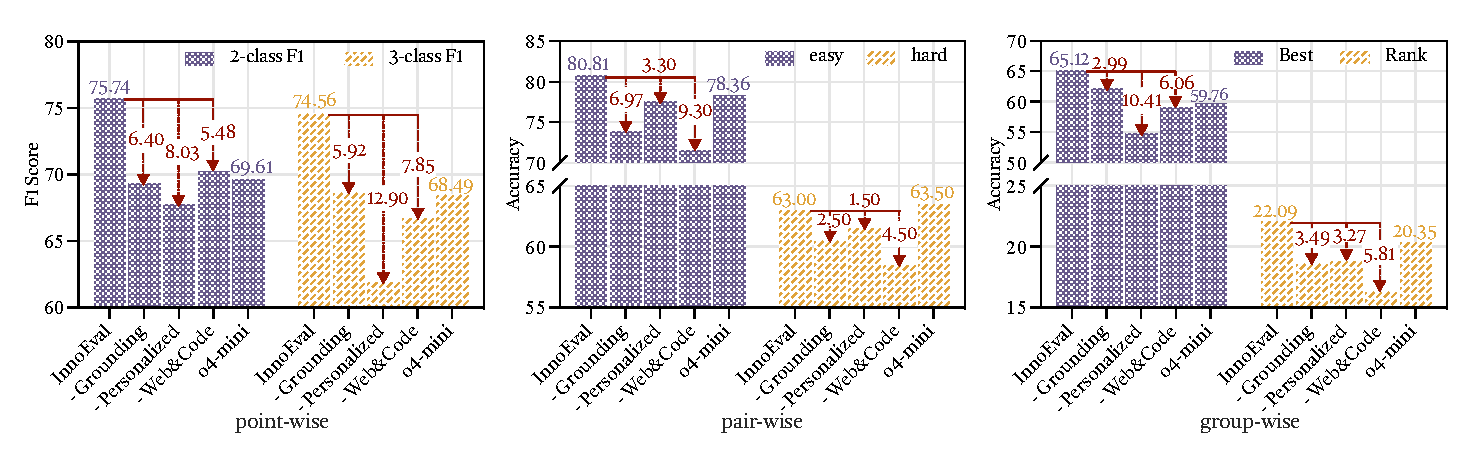
\includegraphics[width=.95\textwidth]{figure/ablation.pdf}
        % \caption{\textbf{Ablation Studies.}}
        \label{fig:ablation}
    \end{subfigure}
    \vskip -0.05in
    \caption{\textbf{Left Heat Map: Human Evaluation}. Correlations between {\ours}'s scores on the five dimensions and the scores assigned by human experts (\textit{Human}), as well as by online peer-review comments (\textit{Reviews}) on the same five dimensions.
    \textbf{Right Bar Charts: Ablation Studies.} -\textit{Grounding} removes the grounding module and feeds raw search results directly into evaluation; -\textit{Personalized} disables the persona, letting the agent evaluate without assumed identity; -\textit{Web\&Code} restricts retrieval to relevant papers only (no web or code search); \textit{o4-mini} swaps the backbone model for o4-mini; \textit{InnoEval} denotes our full configuration.}
    \label{fig:human-ablation}
    \vskip -0.2in
\end{figure*}

\vskip -0.2cm
\subsection{Baselines and Implementation Details}
We select four categories of baselines for a comprehensive comparison with \textbf{\ours}.
\textit{i) Naive method}: \textbf{CoT} and \textbf{RAG};
\textit{ii) Idea generation method}: \textbf{ResearchAgent} \cite{researchagent};
\textit{iii) End-to-end scientific discovery method}: \textbf{InternAgent} \cite{internagent};
And specifically designed \textit{iv) Idea evaluation method}: \textbf{GraphEval} \cite{grapheval} and \textbf{ScholarEval} \cite{scholareval}.
For all baselines, we uniformly adopt DeepSeek-V3.2 \cite{deepseek-v3.2} as the backbone model.
We also test with o4-mini \cite{o4-mini} in \S\ref{sec:ablations} to demonstrate {\ours}'s robustness across different models.
Please refer to Appx.\ref{app:baselines} for more details about the baselines and our reproduction.

\textbf{Implementation.}
We use \texttt{bge-base-en-v1.5} as the retriever and \texttt{bge-reranker-base} as the reranker \cite{bge} for the retrieval in our paper.
At search time, we set the maximum retention number $m$ for each resource type to 10, fix the weight $\alpha$ between semantic score and LLM score at 0.2, and cap the rounds of query refinement $\boldsymbol{N}$ to 3.
The cost of evaluating one sample is 0.42\$.
All the prompts used in our paper can be found in Appx.\ref{app:prompts}.

% \vskip -0.2cm
\section{Experiment Results}

\subsection{Main Results}
\textbf{Quantitative Results.}
As shown in Tab.\ref{tab:main_number}, our {\ours} can achieve state-of-the-art performance compared to other baselines across all tasks.
On the point-wise tasks, we observe label collapse on most baselines: their predictions only concentrate on one or two labels, manifested by F1 scores substantially lower than Accuracy.
Owing to ample evidence support and multi-dimensional, multi-perspective evaluation, our method disperses label predictions and attains F1 scores of 75.74\% and 74.56\%.
This also enables {\ours} to perform better on pair and group tasks.
Since GraphEval is trained only for single-idea label prediction, its performance on pair and group tasks is very poor, highlighting the flexibility requirements of the idea evaluation system.
Additionally, ResearchAgent relies on a pre-constructed literature collection, making its evaluation of relatively new ideas inadequate.
Although InternAgent and ScholarEval design sophisticated search pipelines, due to limitations in search resources and the singularity of evaluation, their evaluation results struggle to align with human labels.

\textbf{Qualitative Results.}
Beyond quantitative tests, we also qualitatively compare the point-wise evaluation quality of {\ours} and other baselines from multiple perspectives using LLM-as-judge, as reported in Tab.\ref{tab:main_llm}.
Our multi-source, in-depth search renders the evaluation results more reasonable (\textit{Rationality}) and well-grounded (\textit{Supportiveness}).
Meanwhile, the multi-dimensional and multi-perspective evaluation paradigm grants our analysis an over 90\% win-rate in \textit{Depth} compared with most methods.
In addition, the improvement suggestions derived from future papers endow our evaluation with stronger \textit{Constructiveness}, with over 80\% win-rate compared with all baselines.
It is worth noting that ScholarEval is a strong baseline, which beats {\ours} on more than 25\% of the samples in terms of \textit{rationality}, \textit{supportiveness}, and \textit{depth}.
Nevertheless, the limited evaluation dimensions and the lack of evidence-based improvement suggestions render its \textit{constructiveness} comparable to that of other baselines.
Overall, the comprehensive and systematic evaluation report produced by {\ours} yields an over 70\% win-rate in \textit{Overall Quality}.

\begin{figure*}
    \begin{subfigure}[b]{0.35\textwidth}
        \centering
        \vskip -0.1cm
        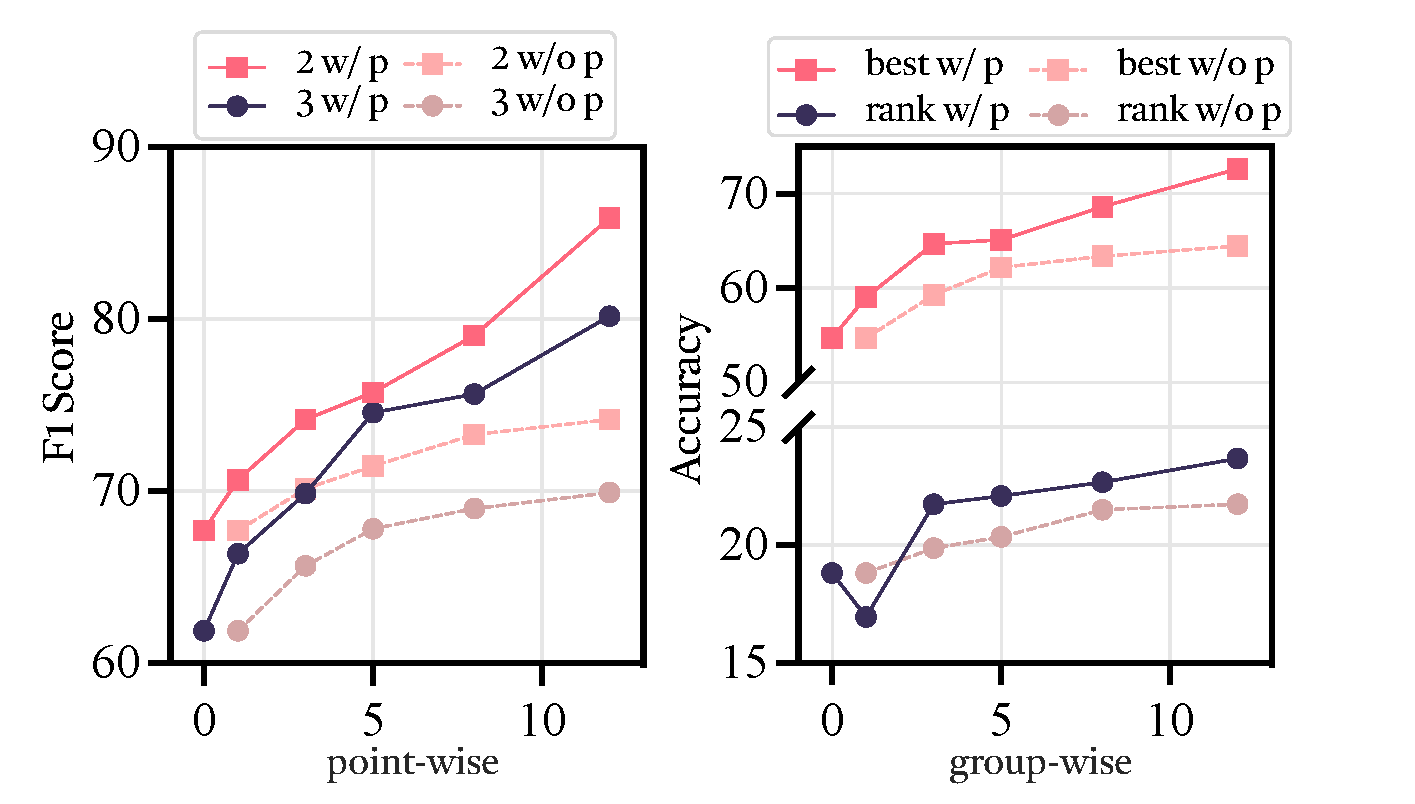
\includegraphics[width=1.\textwidth]{figure/persona.pdf}
        \caption{\textbf{Multi-perspective Test-time Scaling.}}
        \label{fig:persona}
        \vskip -0.2in
    \end{subfigure}
    \begin{subfigure}[b]{0.21\textwidth}
        \centering
        \vskip -0.1cm
        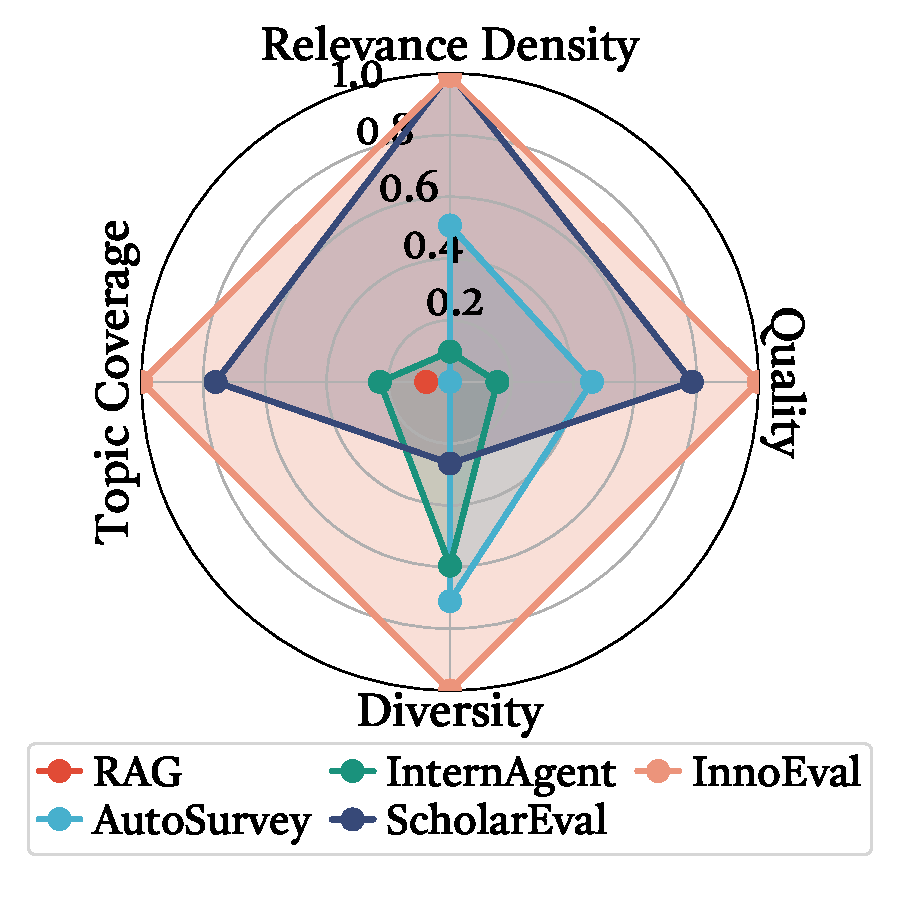
\includegraphics[width=1.\textwidth]{figure/radar_methods.pdf}
        \caption{\textbf{Search Module Eval.}}
        \label{fig:search}
    \end{subfigure}
    \begin{subfigure}[b]{0.21\textwidth}
        \centering
        \vskip -0.1cm
        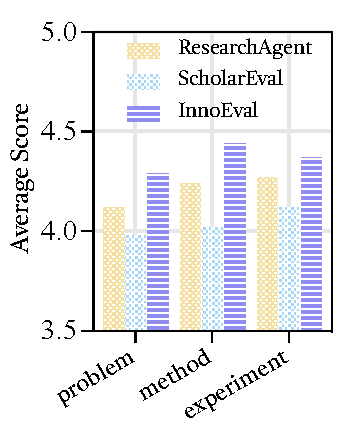
\includegraphics[width=.8\textwidth]{figure/idea_generation.pdf}
        \caption{\textbf{Idea Generation.}}
        \label{fig:idea_generation}
        \vskip -0.2in
    \end{subfigure}
    \begin{subfigure}[b]{0.21\textwidth}
        \centering
        \vskip -0.1cm
        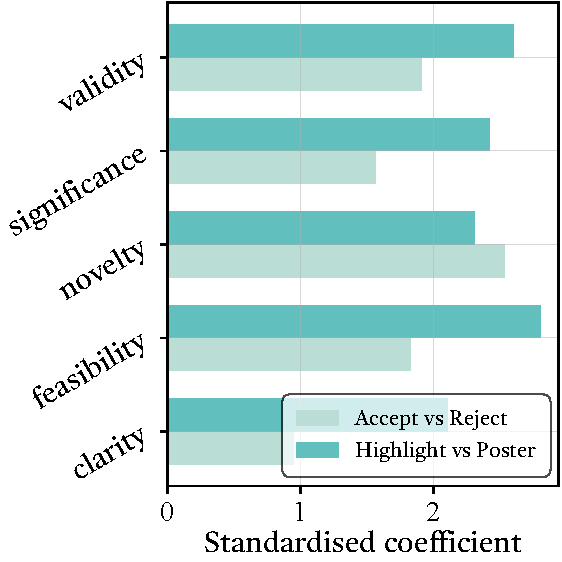
\includegraphics[width=1.\textwidth]{figure/logistic_coef.pdf}
        \caption{\textbf{Metrics Influence.}}
        \label{fig:log_coef}
    \end{subfigure}
    \vskip -0.15cm
    \caption{\textit{(a)} \textbf{Multi-perspective Test-time Scaling.} We compare the test-time scaling results with or without academic personas on point-wise and group-wise tasks. \textit{(b)} \textbf{Search Module Eval.} We compare our heterogeneous deep knowledge search engine with the search modules of other baselines from four metrics. The specific definition of each metric can be found in Appx.\ref{app:search_metrics}. \textit{(c)} \textbf{Idea Generation.} We use the evaluation results of different methods as feedback to improve the idea generation pipeline in ResearchAgent. \textit{(d)} \textbf{Metrics Influence.} We explore critical metrics determining acceptance or highlighting of the idea by linear regression.}
    \label{fig:radar_coef}
    \vskip -0.2in
\end{figure*}

\textbf{Human Evaluation.}
We randomly sample 60 instances from $\boldsymbol{\mathcal{D}}_\textrm{point}$ and have human experts score them on five dimensions under the same rating scheme with {\ours}.
We also prompt an LLM to score them on the five dimensions, conditioned on their ground-truth peer-review comments, to represent real peer reviews.
Detailed evaluation procedures are provided in Appx.\ref{app:human}, with all results shown in Fig.\ref{fig:human-ablation}.
It can be observed that {\ours}'s scores exhibit strong positive correlations with both expert and peer-review judgments across all five dimensions, with correlation coefficients $\ge$ 0.5.
Among the five dimensions, clarity yields the highest correlation, as it solely concerns logical and structural coherence and is therefore relatively straightforward to assess.
In contrast, significance shows relatively lower correlation, reflecting its inherent complexity and thus points to a promising avenue for our future work.

\vskip -0.2cm
\subsection{Ablations}
\label{sec:ablations}
In Fig.\ref{fig:human-ablation}, we illustrate {\ours}'s performance after ablating or replacing key modules.
It can be seen that removing grounding (-\textit{Grounding}) leads to varying degrees of performance degradation across different tasks, indicating that our Grounding Agent can effectively filter out noise in the retrieved reports and enables the evaluation to focus more on relevant information.
Moreover, directly employing LLM-as-Judge (-\textit{Personalized}) causes a marked performance drop, especially on point-wise and group-wise tasks, underscoring that incorporating personalized evaluation effectively mitigates the bias and subjectivity inherent in LLM-as-Judge.
To validate the effectiveness of leveraging diverse retrieval sources, we re-conduct the evaluation using only the literature search results (-\textit{Web\&Code}).
The outcome shows that search richness can significantly improve evaluation accuracy and emphasizes the critical role of sufficient background knowledge in idea assessment.
A finer-grained observation is that restricting retrieval to literature gives more hurt to pair-wise and group-wise tasks, indicating that comparing multiple ideas demands especially rich background knowledge.
We further replace {\ours}'s backbone from DeepSeek-V3.2 with o4-mini.
Despite slight declines on some tasks, we can still surpass the strongest baseline, demonstrating its robustness across different models.

\vskip -0.2cm
\subsection{Analysis}
\textbf{Multi-perspective Test-time Scaling.}
\label{para:persona_scaling}
In Fig.\ref{fig:persona}, we show how {\ours}'s performance varies with the number of different academic personas in evaluation, compared with vanilla Test-Time Scaling (TTS) without personas.
Clear scaling laws are observed under both \textit{w/} and \textit{w/o} persona, demonstrating that increasing generation diversity can effectively enhance evaluation performance.
However, across all task settings, plain TTS consistently underperforms personalized TTS, and as the number of samples increases, the performance gain of vanilla TTS gradually plateaus, whereas personalized TTS maintains robust growth momentum.
This further underscores the importance of reviewer consensus.
Vanilla TTS essentially coerces a single reviewer to fabricate divergent opinions, whereas authentic consensus emerges from reviewers with diverse backgrounds converging after examining the idea from distinct perspectives.
Another interesting phenomenon can corroborate this conclusion.
In group-wise setting, using a single persona underperforms the no-persona baseline on ranking tasks, as the shift from 0 to 1 persona merely transforms the inherent bias of the LLM to that specific persona, without addressing the fundamental issue.
Through this empirical study, it should be noted that our choice of randomly selecting 5 personas in the main experiments balances evaluation efficiency and effectiveness, as a larger pool would sharply increase inference time, but it does not represent the performance ceiling of {\ours}.

\begin{figure*}
    \centering
    \vskip -0.1cm
    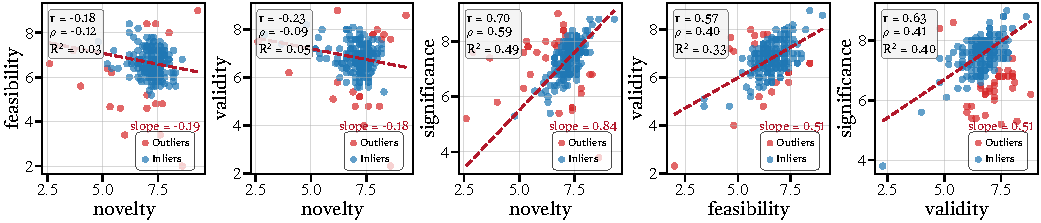
\includegraphics[width=1.\textwidth]{figure/metrics_pairs.pdf}
    \vskip -0.05in
    \caption{\textbf{Scatter Plots Between Metric Pairs.} We perform linear regression fitting for each metric pair. The red dashed line is the fit after removing outliers, and its \textit{slope} is reported. $r$ denotes the Pearson coefficient, $\rho$ is the Spearman coefficient, and R$^2$ represents the fit goodness of all inliers explained by the fitted line. A complete version of all metric pairs' correlation can be seen in Fig.\ref{fig:all_metrics_pair}.}
    \label{fig:metrics_pair}
    \vskip -0.2in
\end{figure*}

\textbf{Effectiveness of Deep Knowledge Search Engine.}
To further demonstrate the effectiveness of our deep knowledge search engine, in Fig.\ref{fig:search} we specially isolate and compare the search engines employed by each baseline, additionally including AutoSurvey \cite{autosurvey}, a baseline specifically designed for literature surveys with a strong retrieval engine.
Although our two strong baselines ScholarEval achieve high relevance, it causes the search results to converge and thereby sacrifice diversity.
AutoSurvey, in pursuit of diverse results, neglects coverage of the idea's topic.
Only our heterogeneous deep knowledge search engine simultaneously preserves relevance, coverage, and diversity.


\textbf{{\ours}'s reviews can serve as an effective reference for idea optimization.}
In Fig.\ref{fig:idea_generation}, we integrate different evaluation methods into the idea iteration pipeline of ResearchAgent (an idea generation method) and rigorously adhere to the ResearchAgent's benchmark and setting to assess the quality of the generated ideas.
The results demonstrate that the actionable revision suggestions provided by {\ours} further boost idea quality throughout the iterative process, yielding significant improvements across problem formulation, methodology, and experimental design compared to the vanilla ResearchAgent.
This improvement is attributed to our multi-dimensional idea evaluation and highly feasible revision feedback in the evaluation reports.
In contrast, ScholarEval's exclusive focus on the contribution and soundness dimensions leads to biased idea optimization, resulting in degraded generation quality.

\textbf{Novelty is the most critical factor in an idea's acceptance, whereas achieving highlight requires well-rounded development across all dimensions.}
In Fig.\ref{fig:log_coef}, we try to explore what is the most critical dimension that determines whether an idea will be accepted or highlighted.
We frame it as a linear regression problem over five evaluation dimensions.
The acceptance of an idea can thereby be cast as a binary classification of \textit{reject} versus other labels (\textit{poster} or \textit{highlight}), while the elevation to highlight can be further reduced to a second binary distinction between \textit{poster} and \textit{highlight}.
We fit a linear regression on $\boldsymbol{\mathcal{D}}_\textrm{point}$ predicted by {\ours} and interpret the resulting coefficient magnitudes as indicators of dimensional importance.
We can see that \textit{novelty} is the most decisive predictor of whether an idea is accepted, a result consistent with human intuition.
\textit{Validity}, \textit{significance}, and \textit{feasibility} are also influential, whereas \textit{clarity} exerts the weakest effect.
However, once the acceptance bar is reached, \textit{feasibility} gains prominence.
This means the focus shifts to whether comprehensive experiments can be designed to demonstrate the proposed methodology.
All remaining dimensions likewise carry substantial weight, indicating that highlight status requires well-rounded strength and underscores the demand for a solid contribution.

\textbf{Mutual relationships among evaluation dimensions.}
To further examine the interrelations among all evaluation dimensions, we plot pairwise scatter plots of all the metrics and fit their linear trends, then quantify their correlations as shown in Fig.\ref{fig:metrics_pair}.
Several interesting findings deserve emphasis:
1) \textit{Significance} exhibits strong positive correlations with both \textit{novelty} and \textit{validity}, indicating that creative ideas grounded in solid theory can exert lasting impacts.
2) \textit{Feasibility} and \textit{validity} are likewise strongly correlated, an expected pattern aligning with human cognition: theoretically well-founded ideas are easier to verify experimentally.
3) \textit{Novelty} shows slight negative correlations with \textit{validity} and \textit{feasibility}, suggesting that more novel ideas are less likely to receive theoretical support or experimental confirmation.
4) Only \textit{clarity} and \textit{significance} exhibit positive correlations with all other metrics, which also makes sense because \textit{clarity} serves as the prerequisite for every other dimension, whereas \textit{significance} relies on the remaining metrics as its foundation.
These observations align well with scholarly cognition, providing convergent evidence that {\ours} can successfully capture the essence of idea evaluation.

\textbf{{\ours} can recognize the real innovation in practice.}
In Appx.\ref{app:case}, we show {\ours}'s evaluation report of a famous idea from ``\textit{Mamba: Linear-Time Sequence Modeling with Selective State Spaces}'' \cite{mamba}.
Our search engine can retrieve key references for Mamba (e.g., S4 \cite{s4}, FlashAttention-V2 \cite{flashattention}, H3 \cite{h3}), relevant discussion blogs from the web, and important code repos related to its experiments (e.g., state-space/s4\footnote{\url{https://github.com/state-spaces/s4}.}).
After fine-grained grounding, reviewers with diverse academic backgrounds and preferences evaluate the idea from multiple perspectives and dimensions, with each dimension containing detailed review comments.
The final meta-review synthesizes all opinions to provide an overall assessment and decision.
Notably, consensus across different perspectives can effectively mitigate biases inherent to single viewpoints (e.g., Reviewer 2), yielding sound decisions and preventing the tragedy of genuinely innovative ideas being overlooked in practice.
Finally, the report includes actionable suggestions for idea improvement from multiple angles, including method, model, experiments, etc.
